\newsavebox{\boxcc}
\Savebox{\boxcc}{
\hspace{-0.25cm}
\begin{minipage}[l]{\columnwidth}
\begin{lstlisting}[style=conescframe]
context group BaseStationG {
*\lstnote{layereddef}* layered command void report(msg_t msg);
}implementation {
*\lstnote{contexts}* contexts Reachable,
*\lstnote{isdefault}*          Unreachable is default,
*\lstnote{iserror}*          MyErrorC is error;
 components Routing, Logging;
 Reachable.Collection -> Routing;
 Unreachable.DataStore -> Logging;}
\end{lstlisting}
\end{minipage}
}
\newsavebox{\boxbscm}
\Savebox{\boxbscm}{
\hspace{-0.25cm}
\begin{minipage}[l]{\columnwidth}
\begin{lstlisting}[style=conescframe]
module BaseStationContextManager {
 uses context group BaseStationG;
}implementation {
 event msg_t Beacon.receive(msg_t msg) {
*\lstnote{actBS}*  activate BaseStationG.Reachable;
  call BSReset.stop(); 
  call BSReset.startOneShot(TIMEOUT);}
 event void BSReset.fired() {
*\lstnote{actNoBS}*  activate BaseStationG.Unreachable;}}
\end{lstlisting}
\end{minipage}
}
\newsavebox{\boxc}
\Savebox{\boxc}{
\hspace{-0.25cm}
\begin{minipage}[l]{\columnwidth}
\begin{lstlisting}[style=conescframe]
context Unreachable {
*\lstnote{dependence}* transitions Reachable iff ActivityG.Running;
 uses interface DataStore;
}implementation {
*\lstnote{activatedUnreachable}* event void activated(){//...}
*\lstnote{deactivatedUnreachable}* event void deactivated(){//...}
*\lstnote{checkUnreachable}* command bool check(){//...}
 layered command void report(msg_t msg){
*\lstnote{layeredimp}*  call DataStore.deposit(msg);}}
\end{lstlisting}
\end{minipage}
}
\newsavebox{\boxirc}
\Savebox{\boxirc}{
\hspace{-0.25cm}
\begin{minipage}[l]{\columnwidth}
\begin{lstlisting}[style=conescframe]
context Reachable {
 uses interface Collection;
 uses context group BatteryG; 
}implementation {
*\lstnote{activated}* event void activated(){ 
  call GPS.stop();}
*\lstnote{deactivated}* event void deactivated(){//...}
*\lstnote{check}* command bool check(){
  return call BatteryG.getContext() == BatteryG.Normal;}
 layered command void report(msg_t msg){
*\lstnote{layeredimp2}*  call Collection.send(msg);}}
\end{lstlisting}
\end{minipage}
}
\newsavebox{\boxlc}
\Savebox{\boxlc}{
\hspace{-0.25cm}
\begin{minipage}[l]{\columnwidth}
\begin{lstlisting}[style=conescframe]
context Low {
*\lstnote{triggers}* triggers BaseStationG.Unreachable;
}implementation {//...}
\end{lstlisting}
\end{minipage}
}
% \newsavebox{\boxmc}
% \Savebox{\boxmc}{
% \hspace{-0.25cm}
% \begin{minipage}[l]{\columnwidth}
% \begin{lstlisting}[style=conescframe]
% configuration ApplicationC {
% }implementation {
% *\lstnote{declaration}* components BaseStationG, Application;
%  //...
% *\lstnote{wiring}* Application.BaseStationG -> BaseStationG;}
% \end{lstlisting}
% \end{minipage}
% }
\newsavebox{\boxmm}
\Savebox{\boxmm}{
\hspace{-0.25cm}
\begin{minipage}[l]{\columnwidth}
\begin{lstlisting}[style=conescframe]
module User {
*\lstnote{cgdecl}* uses context group BaseStationG;
}implementation {
 event void Timer.fired() {
*\lstnote{calling}*  call BaseStationG.report(msg);}
*\lstnote{eventCC}* event void BaseStationG.contextChanged(context_t con) {
*\lstnote{concheck}*  if(con == BaseStationG.Reachable) // DO SOMETHING...}}
\end{lstlisting}
\end{minipage}
}
\newsavebox{\boxnmc}
\Savebox{\boxnmc}{
\hspace{-0.25cm}
\begin{minipage}[l]{\columnwidth}
\begin{lstlisting}[style=conescframe]
context NotMoving {
*\lstnote{transitions}* transitions Resting;
}implementation {//...}
\end{lstlisting}
\end{minipage}
}
\vspace{-0.09in}
\section{ConesC}\label{sec:conesc}

% \conesc provides a design-time support for developing a self-adaptive software,
% which alternates its behavior at run-time including catching and handling
% errors. Along with this, our approach provides a deep modularization, since
% behavioral variations are encapsulated into different modules. The latter, as we
% show in Sec.~\ref{sec:evalcomp}, are highly decoupled, which enhances code
% readability and re-usability as well as debugging and developing processes.

We illustrate how we render the concepts in
Section~\ref{sec:appdesign} within \conesc: our own context-oriented
extension to nesC.  We describe a notion of context module and
configuration in Section~\ref{subsec:components}, and discuss in
Section~\ref{subsec:usage} how programmers use these constructs to
specify an application's adaptive behavior.
Section~\ref{subsec:usage} describes how \conesc programmers deal with
context transitions and their relations.

\subsection{Context Group and Individual Contexts}\label{subsec:components}

\putsnippet{
 caption=Context group in \conesc.,
 label=fig:ccc,
 boxname=boxcc
}

Context groups in \conesc extend the standard nesC
configurations. Programmers use context groups to to declare layered
functions and the contexts providing the corresponding behavioral
variations depending on the situation. 

Fig.~\ref{fig:ccc} shows an example for the \emph{Base-station}
group. A layered \code{report} function is declared on
line~\lstref{layereddef} by using the keyword \code{layered}. The
contexts providing the necessary behavioral variations are specified
following the keyword \code{contexts} on line~\lstref{contexts}. In
this case, programmers define two such contexts, depending on
base-station reachability. The \code{is default} modifier, shown on
line~\lstref{isdefault} indicates what context is active at
start-up. The next \code{is error} modifier on line~\lstref{iserror}
declares context \code{MyErrorC} as an \emph{error} context, which
programmers may optionally use to handle errors during the execution,
as we discuss in Section~\ref{subsec:rules}. If an error context is
not declared, it is generated automatically.

\putsnippet{
 caption=\emph{Reachable} context.,
 label=fig:irc,
 boxname=boxirc
}

\putsnippet{
 caption=\emph{Unreachable} context.,
 label=fig:cc,
 boxname=boxc
}

The individual contexts in \conesc extend the standard nesC modules by providing
context-dependent implementations of layered function declared in context
groups. Only one context at a time can be \emph{active} in a group, meaning the sole implementation of a given layered function can be provided at a time by the
context.

For example, Fig.~\ref{fig:irc} and~\ref{fig:cc} show \conesc snippets
for the \emph{Reachable} and \emph{Unreachable} contexts referenced in
Fig.~\ref{fig:ccc}. They provide different implementations for
\code{report} depending on the situation. If the base-station is
\emph{Reachable}, this the corresponding context is active, the code
transmits the message to the base-station, as in
line~\lstref{layeredimp2} of Fig~\ref{fig:irc}. Differently, the code
deposits a message in local memory as in line~\lstref{layeredimp} of
Fig.~\ref{fig:cc}.

Developer may need to specify operations upon activating a context,
such as initialization of variables or enabling/disabling hardware
modules. For example, on entering the \emph{Reachable} context,
programmers may decide to disable the GPS sensor, as location
information can be inferred from the (static)
base-station. Programmers specify this functionality within the body
of a predefined \code{activated} event, as in
line~\lstref{activatedUnreachable} of Fig.~\ref{fig:irc}. Similarly,
programmers may specify clean-up operations within \code{deactivated}
events, as in line~\lstref{deactivatedUnreachable} of
Fig.~\ref{fig:irc}.  Providing an implementation for these events,
however, is not mandatory.

\subsection{Execution}\label{subsec:usage}

% Context groups encaspulate behavioral variations sharing some common
% characteristic or related to the same funcitonality. Within the
% \emph{Base-station} group of Fig.~\ref{fig:ccc}, for example,
% programmers activate different behavioral variations for function
% \code{report} depending on base-station reachability. 

\putsnippet{
 caption=Base-station context manager.,
 label=fig:bscm,
 boxname=boxbscm
}

Fig.~\ref{fig:bscm} shows a sample snippet of code to detect and to
activate the proper context in the base-station example. Programmers
can, anywhere in the code, trigger explicit changes between contexts
in a group. This is as simple as using the \code{activate} keyword
followed by a full context name. In this fragment of code, the
\emph{Reachable} context is activated on line~\lstref{actBS} as soon
as a beacon from the base station is received. Should the timeout
expire with no more beacons received, context \emph{Unreachable} is
activated on line~\lstref{actNoBS}. Either context change results in a
different context-dependent implementation of \code{report} to be
activated.

\putsnippet{
 caption=User module.,
 label=fig:mm,
 boxname=boxmm
}

Modules using layered functions perform function calls transparently
w.r.t.\ the available contexts and, most importantly, independently of
what context is active at a given moment. Fig.~\ref{fig:mm} shows one
such example where no explicit references appear to which and how many
behavioral variations exist for function \code{report}. Following the
indication that context group \emph{BaseStationG} is used, as
specified on line~\lstref{cgdecl}, the call to the layered function
\code{report} on line~\lstref{calling} refers to the context group and
not to the individual contexts. The net advantage is that the use of
context-dependent functionality, and context detection and activation
are fully decoupled. the two may be implemented even in different
modules.


Nevertheless, should programmers of user modules need to find out
about context changes, a predefined event~\code{contextChanged} is
fired corresponding to every context change, as shown on
line~\lstref{eventCC} in Fig.~\ref{fig:mm}. % This event can be caught
% and handled, as it is shown on the line~\lstref{eventCC} in
% Fig.~\ref{fig:mm}, but it is not mandatory though.
Within the event handler, programmers can access constant values in a
context group that our translator automatically generates, as
described in Section~\ref{sec:translator}, to find out what context
was activated and to react accordingly, as shown on
line~\lstref{concheck}.


% This section shows how ConesC can be used to invoke a behavioral
% variation. Here we describe one aspect of an application's behavioral variation,
% which is related to the Base Station availability. As it was mentioned before,
% if a node receives a beacon from the Base Station it activates the \emph{Reachable}
% context, and the \emph{Unreachable} context in case of timeout.
% Since the behavioral variation is encapsulated in a context group \emph{BaseStationG},
% a developer may not care about the context implementation and use a context group
% Tiny fix.to change a behavior of the application at run-time. Fig.~\ref{fig:mc} depicts the main
% configuration, where the base station group is declared on line~\lstref{declaration} and wired
% as a standard component afterward on the line~\lstref{wiring}.

% \putsnippet{
%  caption=Main configuration.,
%  label=fig:mc,
%  boxname=boxmc
% }

\subsection{Transition Rules}\label{subsec:rules}

\putfigure{caption=Context activation checks.,label=fig:ad}{
 \centering
 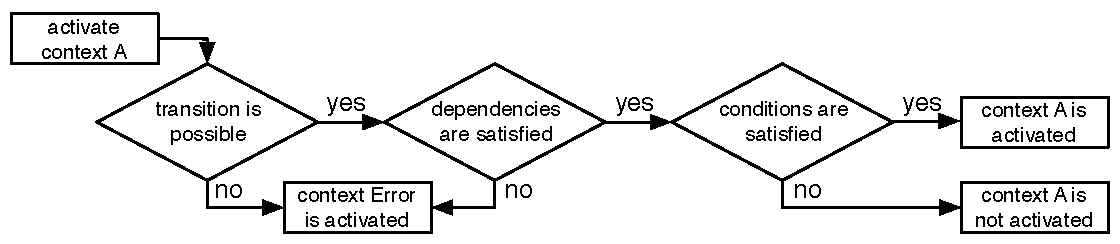
\includegraphics[width=\columnwidth]{pdf/activation_diagram}
}

In general, programmers need to take significant care of context
transitions, in that the latter may drastically change an
application's behavior. To better support programmers in doing so,
every context transition in \conesc entails several checking stages,
as shown in Fig.~\ref{fig:ad}. A successful check allows the
transition to continue, while the failure leads either to the
canceling of the transition or to activation of the \emph{Error}
context. Our translator automatically generates this context unless a
programmer-provided one is explicitly declared in a context group by
using the keyword \code{is error}, as shown on line~\lstref{iserror}
in Fig.~\ref{fig:ccc}.

\putsnippet{
 caption=\emph{NotMoving} context.,
 label=fig:nmc,
 boxname=boxnmc
}

The first check in Fig.~\ref{fig:ad} looks at feasible transitions. In
the context diagram of Fig.~\ref{fig:wtd}, within the \emph{Activity}
group, it is only possible to transition from \emph{NotMoving} to
\emph{Resting}. Feasible transitions are specified within the
individual contexts using the keyword \code{transitions} as in
line~\lstref{transitions} of Fig.~\ref{fig:nmc}. An attempt to
initiate a transition from a given context to one that is not
explicitly listed in the former leads to the activation of the
\emph{Error} context. Indeed, such occurrences typically represent a
significant design or implementation flaw requiring special handling
at run-time, which programmers implement within the \emph{Error} context.

There may also exist relations across context groups. For example,
within the \emph{Base-station} group, a transition from
\emph{Unreachable} to \emph{Reachable} is likely only meaningful if
context \emph{Running} within the \emph{Activity} group is active,
indicating the animal was actually moving when the node gained
base-station connectivity. These inter-group relations are covered in
our design by context dependencies, declared as shown on
line~\lstref{dependence} in Fig.~\ref{fig:cc}. Within the
\code{transitions} clause, the keyword \code{iff} is optionally
employed to indicate the full name of another context whose activation
is required to perform the given transition. The second check in
Fig.~\ref{fig:ad} verifies this rule, again leading to the
\emph{Error} context in case of violations to give programmers an
explicit chance to handle the situation.

The last check in Fig.~\ref{fig:ad} considers violations to ``soft''
requirements that do not necessarily indicate a design or
implementation flaw. Rather, such requirements may be simply needed
for efficiently executing the functionality in a context. For example,
before activating the \emph{Reachable} context, programmers may want
to check that sufficient energy is available to invest in bulk data
transfers to the base-station. Should this not be the case, they may
defer the activation of the \emph{Reachable} context until the solar
panels gather sufficient energy. To implement such processing, \conesc
programmers specify the proper conditions in the body of a predefined
\code{check} command, as shown in line~\lstref{check} of
Fig.~\ref{fig:irc}. If \code{check} returns false, the initiated
context transition does not occur, and the system remains in the
previous context.

\putsnippet{
 caption=\emph{Low} context.,
 label=fig:lc,
 boxname=boxlc
}

Dually, programmers may need to proactively initiate context
transitions as the result of other contexts being activated. The
scenario is symmetric to the previous one: if the base-station is
\emph{Reachable}, but a context transition is initiated to context
\emph{Low} in the \emph{Battery} group of Fig.~\ref{fig:wtd}, the
available energy is running low and it is probably better to refrain
from radio communications even though the base-station is within the
communication range. This makes sure the node does not completely turn
off before the solar panels re-gain energy. Our design allows
programmers to express this processing by using the \code{triggers}
keyword, as shown on line~\lstref{triggers} in Fig.~\ref{fig:lc}. The
\code{triggers} keyword references a context that is to be activated
as the result of the enclosing context being activated. The same
checks shown in Fig.~\ref{fig:ad} apply to this type of transitions as
well.


% Other types of inter-group relations imply automatic triggering of
% context transition. Considering \emph{Battery} group in our example,
% we can notice that for further energy saving developers may want to
% trigger a transition to \emph{Unreachable} context within the
% \emph{Base Station} group as long as \emph{Low} context is active.



%%% Local Variables: 
%%% mode: latex
%%% TeX-master: "bare_conf"
%%% End: 
